\documentclass{article}
\usepackage[top=0pt,left=0pt,bottom=0pt,right=0pt,paperwidth=3.43cm,paperheight=6cm]{geometry}
\usepackage{tikz}
\usepackage{desat}
\pagestyle{empty}
\begin{document}
\centering%
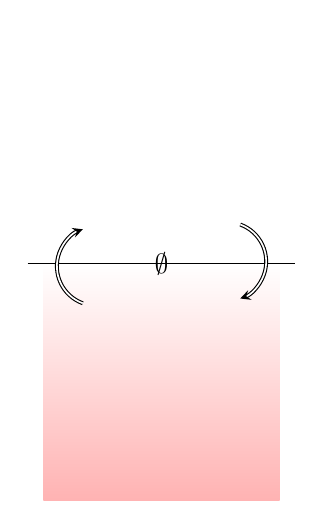
\begin{tikzpicture}[
  echange/.style={-stealth,double=white},
  big echange/.style={echange, double=white, thick}]
\path[use as bounding box] (-1.7,-4.5) rectangle (1.7,1.5);
\tikzair{15}
\shade[top color=white,bottom color=red!30] (-1.5,-4.5) rectangle ++(3,3);
\begin{scope}[yshift=-3cm]
\tikzair{15}
\end{scope}
\draw (-1.7,-1.5) -- ++(3.4,0);
\draw[echange] (1,-1) arc(70:-70:5mm);
\draw[echange] (-1,-2) arc(-110:-250:5mm);
\node at (0,-1.5) {$\emptyset$};
\end{tikzpicture}
\end{document}
